\chapter{Desenvolvendo o primeiro projeto com o MDArte}

Neste capítulo iremos construir um projeto básico usando o MDArte. O projeto
consistirá de um sistema web simples para administrar um ambiente acadêmico,
onde poderemos cadastrar cursos e gerenciar suas informações, bem como inserir
alunos, inscrevê-los nos e gerenciar suas informações.

\section{Criação de um Novo Projeto e Configuração do ambiente}

O plugin do MDArte para o Maven já possui um procedimento parametrizado para
criação de projetos, que funciona como um wizard, onde o usuário deve responder
a perguntas. Através das respostas fornecidas, o MDArte direcionará a criação da
estrutura básica e dos artefatos básicos de configuração de projetos. O
procedimento para criação de um novo projeto é:

\begin{enumerate}
\item Abra o terminal (command prompt) e vá para o diretório onde se deseja
criar o projeto. Na verdade, o projeto será gerado em um subdiretório do
diretório escolhido.

\item Digite o comando: \texttt{maven andromdapp:generate}

\item As perguntas devem ser respondidas de acordo com o projeto a ser
desenvolvido. Abaixo as respostas adequadas para o exemplo desenvolvido neste
capítulo (perguntas em negrito):

\textbf{Please enter your first and last name (i.e. Rodrigo Salvador):} \\
MDArte\\
\textbf{Please enter the name of your J2EE project (i.e. Sistema Academico):}\\
Sistema Academico\\
\textbf{Please enter the id for your J2EE project (i.e. sistemaacademico):}\\
sistemaacademico\\
\textbf{Please enter a version for your project (i.e. 1.0):}\\
1.0\\
\textbf{Please enter the base package name for your J2EE project (i.e. br.mdarte.exemplo.academico):}\\
br.mdarte.exemplo.academico\\
\textbf{Would you like to enable security? (enter 'yes' or 'no')?}\\
yes\\
\textbf{Would you like to use oAuth (enter 'yes' or 'no') ?}\\
no\\
\textbf{Would you like to use MDArte's default Controle Acesso (enter 'yes' or
'no') ?}\\
yes\\
\textbf{Would you like to use modules (enter 'yes' or 'no')?}\\
yes\\
\textbf{Please enter the EJB version number (enter '2' or '3'):}\\
3\\
\textbf{Please enter the Struts version number (enter '1' or '2'):}\\
2\\
\textbf{Would you like to enable the JUnit support for general testing? (enter
'yes' or 'no')? }\\
 no\\
\textbf{Please enter the database backend for the persistence layer: (enter
'hypersonic' or 'mysql' or 'oracle' or 'postgres')}\\
 postgres\\
 
\item Após receber as respostas, o MDArte criará um subdiretório onde será
gerada a estrutura inicial do projeto. A partir desse momento chamaremos esse
diretório de <DiretorioProjeto>.

\item Ainda no console, vá para o diretório onde está seu projeto:
<DiretorioProjeto>.

\item Digite maven. Isto obrigará o Maven a obter todos os artefatos (por
exemplo, bibliotecas) de que o projeto dependerá.

\end{enumerate}

\section{Controle de Acesso}

Neste tutorial estaremos utilizando funcionalidades de controle de acesso, porém
não é nosso propósito explorar suas funcionalidades. Assim, estaremos utilizando
um projeto de controle de acesso desenvolvido pela comunidade do MDArte.

O projeto pode ser obtido a partir do repositório Git do MDArte, pelo endereço
\texttt{https://github.com/MDArte/controleacesso.git} . Por fim, edite também o
arquivo \texttt{project.properties} do ControleAcesso para configurar o tipo de
Banco de Dados a ser utilziado, conforme realizado com o projeto
SistemaAcademico. Note que a propriedade dataSource.name está definida como
controleacessoDS.

Novamente, precisaremos criar um arquivo de configuração do Banco de Dados,
localizado no diretório
\texttt{\textdollar{}JBOSS\_HOME/server/default/deploy/}. O nome do arquivo deve
seguir a mesma formatação mencionada, terminando em -ds.xml (ex.:
\texttt{aplicacoes-ds.xml}), podendo estar no mesmo arquivo com as configurações
do projeto SistemaAcademico.

Exemplo:

\begin{framed}
	\lstinputlisting[language=xml]{files/ControleAcesso-ds.xml}
\end{framed}

Note que no exemplo anterior o ControleAcesso estará utilizando a mesma base de
dados do projeto SistemaAcademico, definida pela tag <connection-url>. Agora,
execute os seguinte comandos, na raiz do projeto ControleAcesso, para gerar,
compilar e copiar os pacotes para o diretório \texttt{\textdollar{}JBOSS\_HOMEHOME/server/default/deploy/}:

\begin{framed}
	\lstinputlisting[language=bash]{files/compila-ca}
\end{framed}

\section{Modelando o nosso primeiro projeto}

Vamos começar agora a modelar o nosso exemplo, mostrando o quão rápido e simples
pode ser usar o MDArte e todo o seu poder de geração.

Para esta parte do tutorial usaremos o MagicDraw. Na barra de ferramentas do
MagicDraw, clicaremos em \texttt{Open Project} e abriremos o xml do projeto,
\texttt{SistemaAcademico.xml} no caminho
\texttt{<DiretorioProjeto>/mda/src/uml/}.

\subsection{Modelando a camada de domínio}
Na camada de domínio, estarão as classes do domínio da aplicação. Elas serão
entidades e estarão associadas a algum modo de persistência. Afim de
contornar os problemas provenientes da utilização de bancos de dados relacionais
em conjunto com o paradigma de orientação à objeto, o MDArte usa o framework
Hibernate\footnote{\hypertarget{http://hibernate.org/orm/}{http://hibernate.org/orm/}}
para gerenciar esta camada.

As classes da camada de domínio deverão conter o estereótipo «Entity» e os
atributos que serão persistidos. Todas as classes de entidade devem
obrigatoriamente estar no pacote <PacoteProjeto>.cd, em que <PacoteProjeto> é o
pacote definido para o projeto.

Neste exemplo, especificamente, iremos também marcar nossas entidades com o
estereótipo «Manageable», tal marcação diz para o MDArte que desejamos que seja
gerado um CRUD padrão para tais entidades, sem a necessidade de modelarmos o
mesmo diretamente.

\begin{enumerate}
\item Crie a mesma estrutura de pacotes que foi definida na criação do projeto.
Dentro da estrutura, crie o pacote “cd”. Podemos ver o resultado na imagem
~\ref{cria_estrutura_pacotes}. 
\begin{figure}[!htb]
	\centering
	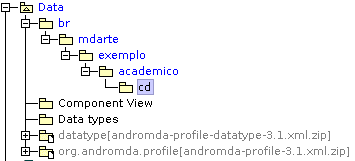
\includegraphics[width=250pt,height=100pt]{imgs/tutorial-mdarte-0000.png}
	\caption{Criação da estrutura de pacotes do projeto e do pacote cd.}
	\label{cria_estrutura_pacotes}
\end{figure}
\item Clique com o botão direito do mouse no pacote “cd” e selecione a opção New
Diagram.Em seguida, selecione Class Diagram. Como mostra a
Figura~\ref{cria_diagrama_classe}.
\begin{figure}[!htb]
	\centering
	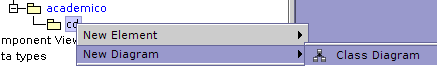
\includegraphics[width=400pt,height=60pt]{imgs/tutorial-mdarte-0001.png}
	\caption{Criação do diagrama de classes da camada de domínio.}
	\label{cria_diagrama_classe}
\end{figure}
	
\item Indique o nome desejado para o diagrama (ex: Entidades).
	
\item No diagrama de classe, crie uma nova classe. Clique com o botão direto
sobre a classe e selecione a opção Specification. Defina o nome da classe como
“Estudante”.
	
\item Crie os atributos na classe Estudante (matricula, nome) selecionando a aba
Attributes e clicando no botão Add. A figura abaixo exemplifica a criação do
atributo matricula. O campo Visibility deve ser public. Não é necessário modelar
o atributo id, pois ele é gerado automaticamente. Como mostra a
Figura~\ref{config_parametro}.

\begin{figure}[!htb]
	\centering
	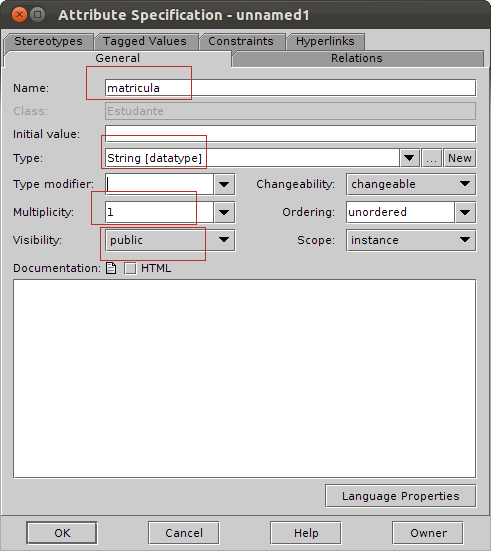
\includegraphics[width=350pt,height=400pt]{imgs/tutorial-mdarte-0002.png}
	\caption{Configuração do parâmetro matrícula da classe Estudante.}
	\label{config_parametro}
\end{figure}
		
A multiplicidade com valor 1 (campo Multiplicity) indica que o atributo é
obrigatório (NOT NULL), já o valor 0..1 indica que o atributo não é obrigatório.
Por padrão, todos os atributos são gerados como NOT NULL.

\item Coloque o estereótipo «Unique» no atributo matricula para indicar que cada
código deve ser único, ou seja, não pode haver duas matrículas iguais. Abra a
especificação do atributo matricula e selecione a aba Stereotypes. Nessa aba
selecione o estereótipo «Unique», como na figura
~\ref{add_estereotipo_matricula}.

\begin{figure}[!htb]
	\centering
	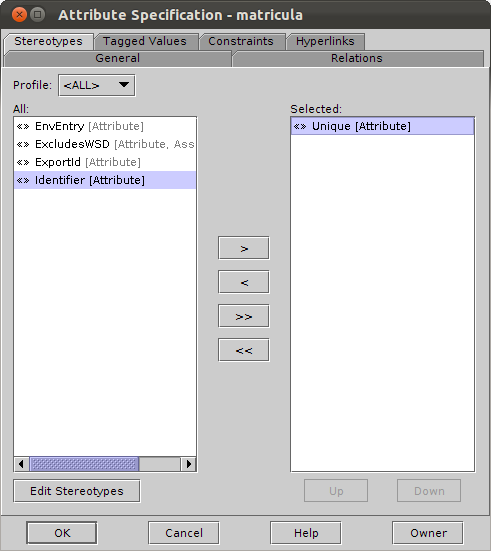
\includegraphics[width=350pt,height=400pt]{imgs/tutorial-mdarte-0003.png}
	\caption{Adição de estereótipo no atributo matrícula.}
	\label{add_estereotipo_matricula}
\end{figure}
	
\item Coloque os estereótipos «Entity» e «Manageable» na classe Estudante, como
na figura ~\ref{add_estereotipo_estudante}. 
\begin{figure}[!htb]
	\centering
	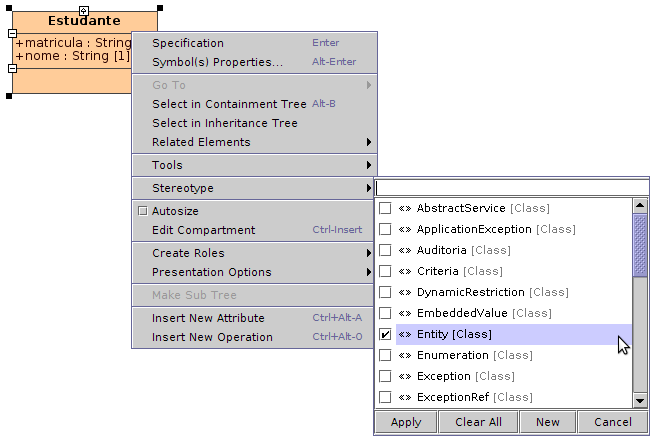
\includegraphics[width=400pt,height=300pt]{imgs/tutorial-mdarte-0004.png}
	\caption{Adição dos estereótipos Entiti e Manageable na classe estudante.}
	\label{add_estereotipo_estudante}
\end{figure}
	
\item No mesmo diagrama de classes, crie outra classe. Clique com o botão direto
sobre a classe e selecione a opção Specification. Defina o nome da classe como
“Curso”.
	
\item Crie os atributos na classe Curso (codigo, nome) selecionando a aba
Attributes e clicando no botão Add. O campo Visibility deve ser public, assim
como feito anteriormente.

\item Coloque o estereótipo «Unique» no atributo codigo para indicar que cada
código deve ser único. Abra a especificação do atributo codigo e selecione a aba
Stereotypes. Nessa aba selecione o estereótipo «Unique».
	
\item Coloque o estereótipo «Entity» na classe.
	
\item Agora, crie uma associação entre as classes. Vá no diagrama de classes e
puxe uma relação Association de uma classe para outra.
	
\item A associação será de 1 para muitos. Assim, clique duas vezes na associação
e irá aparecer a tela de especificação. Edite os campos Multiplicity definindo
valor “0..*” para a entidade Estudante e “1” para a entidade Curso, como na
figura ~\ref{define_multiplicidade_associacao}.
\begin{figure}[!htb]
	\centering
	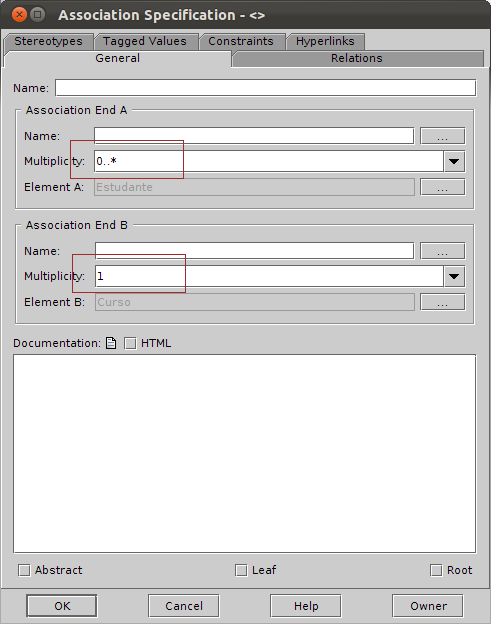
\includegraphics[width=350pt,height=400pt]{imgs/tutorial-mdarte-0005.png}
	\caption{Definindo multiplicidade da associação.}
	\label{define_multiplicidade_associacao}
\end{figure}
	
\item A associação deve ser dupla, tanto Estudante quanto Curso devem ser
visíveis. Dessa forma, mantenha a checkbox Navigable marcada na associação para
as duas classes. Para isso, clique no botão “...” (reticências) da tela
anterior, como na imagem ~\ref{config_navigable_associacao}.
\begin{figure}[!htb]
	\centering
	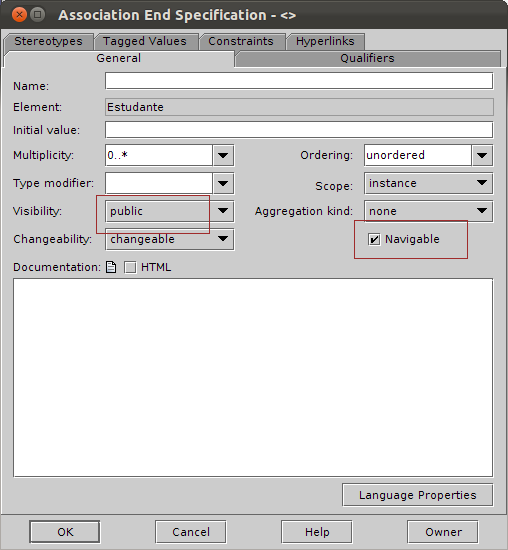
\includegraphics[width=350pt,height=400pt]{imgs/tutorial-mdarte-0006.png}
	\caption{Configuração da navegabilidade da associação.}
	\label{config_navigable_associacao}
\end{figure}
		
O resultado final pode ser visto na imagem ~\ref{resultado_diagrama_classe}: \hfill
\begin{figure}[!htb]
	\centering
	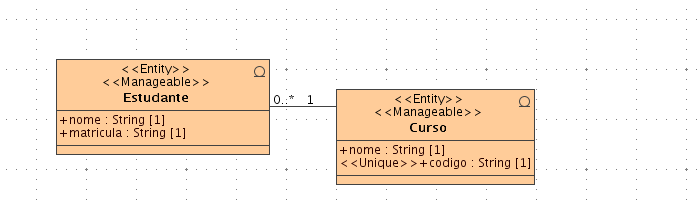
\includegraphics[width=500pt,height=200pt]{imgs/tutorial-mdarte-0007.png}
	\caption{Resultado final da modelagem da camada de domínio.}
	\label{resultado_diagrama_classe}
\end{figure}
	
\item No diretório da aplicação, execute o comando maven para validar o modelo e
gerar o script SQL de criação do Banco de Dados. O resultado apresentado deve
ser “BUILD SUCCESFULL”.
	
\item Observe que dois novos arquivos xml terão sido criados no caminho
\texttt{<DiretorioProjeto>/mda/src/uml/} com os nomes
\texttt{sistemaacademico-geral-Curso.xml} e
\texttt{sistemaacademico-geral-Estudante.xml} , com os crud default gerados pelo
MDArte.

Para compilar e gerarmos estes módulos separados executaremos os comandos:
	
\begin{framed}
	\lstinputlisting[language=bash]{files/compila-cruds}
\end{framed}

\end{enumerate}

\subsection{Criando o Banco de Dados}

Durante a execução do comando maven, todas as classes são criadas
automaticamente. Além disso, também é gerado o código SQL de criação de tabelas
do Banco de Dados. O script SQL pode ser encontrado em
\texttt{<DiretorioProjeto>/core/cd/target/schema-create.sql}. Abrindo o arquivo
é possível notar a presença de comandos de crição das tabelas ESTUDANTE e CURSO.

Execute o conteúdo do arquivo no Banco de Dados utilizado.

Como exemplificação dos casos de usos que serão elaborados por este documento,
execute o seguinte script SQL para criar a base inicial. Note que o script foi
escrito para PostgreSQL e deve ser adaptado para o Banco de Dados escolhido.

\begin{framed}
	\lstinputlisting[language=sql]{files/exemplo.sql}
\end{framed}

\subsection{Modelando a camada de serviços}

Na camada de serviço serão implementadas as classes responsáveis pela lógica de
negócio da aplicação. As classes especificadas se tornarão os serviços (API) da
aplicação. Os serviços definidos no modelo se tornarão disponíveis através de
Session Beans.

Os Session Beans são componentes de negócio. A lógica de negócio dos componentes
EJB se encontram nestes componentes. Existem dois tipos de Componentes Session
Bean, o Stateless Session Bean e o Stateful Session Beans. O Stateless é um
componente de negócio que não mantém conversação com o usuário, não há garantia
que chamadas sucessivas de métodos remotos vão ser feitas no mesmo objeto. O
Stateful é um componente que mantêm estado, com ele temos a garantia que
chamadas sucessivas de métodos remotos feitas por um mesmo cliente serão
processadas por um mesmo objeto.

Os beans EJB precisam ser modelados em um diagrama de classes. As classes destes beans precisam ter o estereótipo «Service». Todas as classes de serviço devem estar no pacote <PacoteProjeto>.cs, em que <PacoteProjeto> é o pacote definido para o projeto.

\begin{enumerate}
\item Crie um pacote <PacoteProjeto>.cs.estudante. Clique então com o botão
direito sobre a pasta estudante, na opção Stereotype, selecione o estereótipo
 «ModuloServico» e clique em Apply. O resultado pode ser visto na imagem
 ~\ref{cria_pacote_servico}:
 \begin{figure}[!htb]
	\centering
	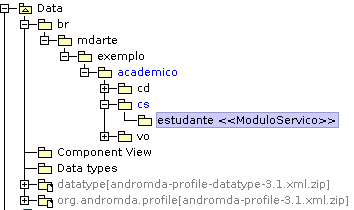
\includegraphics[width=200pt,height=200pt]{imgs/tutorial-mdarte-0008.png}
	\caption{Criação do pacote para a camada de serviço.}
	\label{cria_pacote_servico}
\end{figure} 
	
\item Crie um diagrama de classe dentro do pacote estudante, com o nome que desejar.
	
\item Crie uma classe com nome EstudanteHandler e estereótipo «Service». A
classe EstudanteHandler deve ficar como na figura ~\ref{cria_sevico_estudante}.
\begin{figure}[!htb]
	\centering
	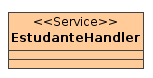
\includegraphics[width=150pt,height=120pt]{imgs/tutorial-mdarte-0009.png}
	\caption{Criação da classe de serviço EstudanteHandler.}
	\label{cria_sevico_estudante}
\end{figure} 
	
\item Crie uma classe com nome EstudanteException e estereótipo
«ApplicationException», como na imagem ~\ref{cria_estudante_exception}.
\begin{figure}[!htb]
	\centering
	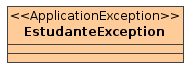
\includegraphics[width=150pt,height=120pt]{imgs/tutorial-mdarte-0010.png}
	\caption{Criação da classe estudante exception.}
	\label{cria_estudante_exception}
\end{figure}
	
\item Arraste para o diagrama de classes recém criado no pacote estudante a classe Estudante.
	
\item Crie uma relação de dependência entre as classes EstudanteHandler e
Estudante, assim como entre EstudanteHandler e EstudanteException. Para isso,
utilize a opção do MagicDraw ilustrada na figura abaixo. Clique na opção, depois
clique na classe, ou método, de origem e arraste a seta até a classe destino,
como na imagem ~\ref{cria_dependencia_servico}.

\begin{figure}[!htb]
	\centering
	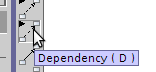
\includegraphics[width=110pt,height=90pt]{imgs/tutorial-mdarte-0012.png}
	\caption{Criação da dependência entre as classes do serviço.}
	\label{cria_dependencia_servico}
\end{figure}

\item Verifique se o diagrama está como a figura
~\ref{resultado_diagrama_classe_servico}.
\begin{figure}[!htb]
	\centering
	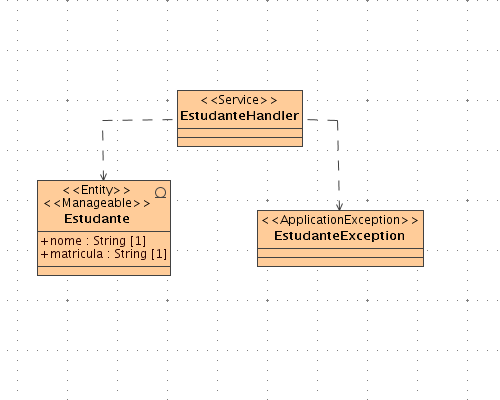
\includegraphics[width=300pt,height=350pt]{imgs/tutorial-mdarte-0011.png}
	\caption{Diagrama de classe completo do módulo de serviço para a classe
	Estudante.}
	\label{resultado_diagrama_classe_servico}
\end{figure}

\item A dependência entre EstudanteHandler e EstudanteException fará com que todos os métodos de EstudanteHandler possam lançar a exceção EstudanteException. Se a dependência tivesse sido entre algum método de EstudanteHandler e não com a própria classe, somente o método com dependência poderia lançar a exceção.

A dependência entre EstudanteHandler e Estudante cria os métodos de acesso ao banco na classe de serviço.

\item Agora faça o mesmo para criar um modulo de serviço para a classe Estudante.
	
\item No diretório da aplicação, execute o comando maven para validar o modelo e gerar as classes de serviço. O resultado apresentado deve ser “BUILD SUCCESSFULL”.
\end{enumerate}

\section{Implementando as classes de controle dos cruds gerados}

Nessa seção vamos implementar as classes de controle dos casos de uso gerados. Para isso, abriremos os arquivos <nomeCasoDeUso>ControleImpl.java. Esses arquivos são pontos de implementação onde deve ser concentrado todo o código que se queira adicionar manualmente às classes de controle. Como tais arquivos só são gerados caso ainda não existam, o código colocado neles não será sobrescrito, ao contrario do que ocorre se inserirmos manualmente codigo nos arquivos <nomeCasoDeUso>Controle.java .

De acordo com os casos de uso gerados automaticamente pelo gerador de cruds do MDArte, iremos implementar respectivamente os seguintes código nos seguintes arquivos, que devem portanto ser abertos no Eclipse ou em outra IDE desejada:

\begin{enumerate}
\item ConsultaEstudanteControleImpl.java :
\begin{framed}
	\lstinputlisting[language=java]{files/ConsultaEstudanteControleImpl.java}
\end{framed}
		
\item MantemEstudanteControleImpl.java :
\begin{framed}
	\lstinputlisting[language=java]{files/MantemEstudanteControleImpl.java}
\end{framed}

\item DetalhaEstudanteControleImpl.java:
\begin{framed}
	\lstinputlisting[language=java]{files/DetalhaEstudanteControleImpl.java}
\end{framed}

\item ConsultaCursoControleImpl.java :
\begin{framed}
	\lstinputlisting[language=java]{files/ConsultaCursoControleImpl.java}
\end{framed}

\item MantemCursoControleImpl.java :
\begin{framed}
	\lstinputlisting[language=java]{files/MantemCursoControleImpl.java}
\end{framed}

\item DetalhaCursoControleImpl.java :
\begin{framed}
	\lstinputlisting[language=java]{files/DetalhaCursoControleImpl.java}
\end{framed}

\end{enumerate}

Agora, no terminal, no <DiretorioProjeto> executaremos o seguinte comando :

\begin{framed}
	\lstinputlisting[language=bash]{files/compile-deploy}
\end{framed}

Abriremos agora o eclipse, daremos Start no servidor jboss e verificaremos então
no navegador o resultado do nosso sistema.
